\chapter{Cypherpunks Write Code}
\label{les:20}

\begin{chapquote}{Lewis Carroll, \textit{Alice in Wonderland}}
``I see you're trying to invent something.''
\end{chapquote}

Like many great ideas, Bitcoin didn't come out of nowhere. It was made
possible by utilizing and combining many innovations and discoveries in
mathematics, physics, computer science, and other fields. While
undoubtedly a genius, Satoshi wouldn't have been able to invent Bitcoin
without the giants on whose shoulders he was standing on.

\begin{quotation}
``He who only wishes and hopes does not interfere actively with the
course of events and with the shaping of his own destiny.''
\end{quotation}
% > <cite>[Ludwig Von Mises]</cite>

One of these giants is Eric Hughes, one of the founders of the
cypherpunk movement and author of the [cypherpunk manifesto]. It's hard
to imagine that Satoshi wasn't influenced by this manifesto. It speaks
of many things which Bitcoin enables and utilizes, such as direct and
private transactions, electronic money and cash, anonymous systems, and
defending privacy with cryptography and digital signatures.

\begin{quotation}
``Privacy is necessary for an open society in the electronic age.
[...] Since we desire privacy, we must ensure that each party to a
transaction have knowledge only of that which is directly necessary
for that transaction. [...]
Therefore, privacy in an open society requires anonymous transaction
systems. Until now, cash has been the primary such system. An
anonymous transaction system is not a secret transaction system.
[...]
We the Cypherpunks are dedicated to building anonymous systems. We are
defending our privacy with cryptography, with anonymous mail
forwarding systems, with digital signatures, and with electronic
money.
Cypherpunks write code.''
\end{quotation}
% > <cite>[Eric Hughes][cypherpunk manifesto]</cite>

Cypherpunks do not find comfort in hopes and wishes. They actively
interfere with the course of events and shape their own destiny.
Cypherpunks write code.

Thus, in true cypherpunk fashion, Satoshi sat down and started to write
code. Code which took an abstract idea and proved to the world that it
actually worked. Code which planted the seed of a new economic reality.
Thanks to this code, everyone can verify that this novel system actually
works, and every 10 minutes or so Bitcoin proofs to the world that it is
still living.

\begin{figure}
  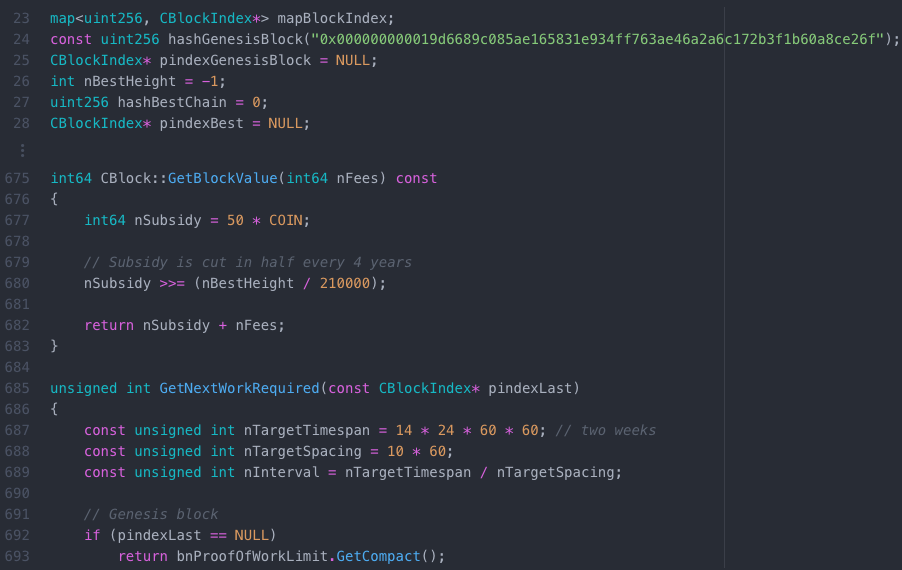
\includegraphics{assets/images/bitcoin-code.png}
  \caption{Code excerpts from Bitcoin version 0.1.0}
  \label{fig:bitcoin-code}
\end{figure}

To make sure that his innovation transcends fantasy and becomes reality,
Satoshi wrote code to implement his idea before he wrote the whitepaper.
He also made sure [not to delay] any release forever. After all,
"there's always going to be one more thing to do."

\begin{quotation}
``I had to write all the code before I could convince myself that I
could solve every problem, then I wrote the paper.''
\end{quotation}
% > <cite>[Satoshi Nakamoto][6]</cite>

In today's world of endless promises and doubtful execution, an exercise
in dedicated building was desperately needed. Be deliberate, convince
yourself that you can actually solve the problems, and implement the
solutions. We should all aim to be a bit more cypherpunk.

\paragraph{Bitcoin taught me that cypherpunks write code.}

% ---
%
% #### Down the Rabbit Hole
%
% - [A Cypherpunk's Manifesto][cypherpunk manifesto] by Eric Hughes
% - [Bitcoin version 0.1.0 announcement][version 0.1.0] by Satoshi Nakamoto
% - [Bitcoin P2P e-cash paper announcement][mail-announcement] by Satoshi Nakamoto
%
% [mail-announcement]: http://www.metzdowd.com/pipermail/cryptography/2008-October/014810.html
% [Ludwig Von Mises]: https://mises.org/library/human-action-0/html/pp/613
% [cypherpunk manifesto]: https://www.activism.net/cypherpunk/manifesto.html
% [version 0.1.0]: https://bitcointalk.org/index.php?topic=68121.0
% [not to delay]: https://bitcointalk.org/index.php?topic=199.msg1670#msg1670
% [6]: http://www.metzdowd.com/pipermail/cryptography/2008-November/014832.html
%
% <!-- Wikipedia -->
% [alice]: https://en.wikipedia.org/wiki/Alice%27s_Adventures_in_Wonderland
% [carroll]: https://en.wikipedia.org/wiki/Lewis_Carroll
